\documentclass[conference]{IEEEtran}
\IEEEoverridecommandlockouts

\usepackage{cite}
\usepackage{amsmath,amssymb,amsfonts}
\usepackage{algorithmic}
\usepackage{graphicx}
\usepackage{textcomp}
\usepackage{xcolor}
\usepackage{booktabs}
\usepackage{multirow}
\usepackage{url}
\usepackage{microtype}
\usepackage{balance}

\setlength{\textfloatsep}{5pt plus 1pt minus 1pt}
\setlength{\floatsep}{5pt plus 1pt minus 1pt}
\setlength{\intextsep}{5pt plus 1pt minus 1pt}
\setlength{\abovecaptionskip}{2pt plus 1pt minus 1pt}
\setlength{\belowcaptionskip}{1pt plus 1pt minus 1pt}
\renewcommand{\baselinestretch}{0.94}

\def\BibTeX{{\rm B\kern-.05em{\sc i\kern-.025em b}\kern-.08em
    T\kern-.1667em\lower.7ex\hbox{E}\kern-.125emX}}

\begin{document}

\title{A Comparative Empirical Study of Lightweight Machine Learning Classifiers for SMS Spam Detection Under Controlled Experimental Conditions}

\author{\IEEEauthorblockN{Pranav Akshit}
\IEEEauthorblockA{\textit{School of Computer Science} \\
\textit{University of Petroleum and Energy Studies (UPES)}\\
Dehradun, Uttarakhand, India \\
Email: student@upes.ac.in}
}

\maketitle

\begin{abstract}
Short Message Service (SMS) remains an indispensable global telecommunication medium, yet its ubiquity has made it a primary conduit for unsolicited spam, financial fraud, and credential-harvesting smishing attacks. While deep neural networks have achieved strong detection scores, their substantial memory footprint, high computational latency, and battery drain impede practical deployment on resource-constrained mobile and edge devices. Conversely, classical machine learning classifiers offer lightweight alternatives, but prior comparative literature suffers from fragmented reporting, uncalibrated single-split evaluations, and unverified preprocessing assumptions. In this paper, we present a rigorously controlled, leakage-free empirical benchmark comparing three classical classifiers---Multinomial Naive Bayes (MNB), Logistic Regression (LR), and Linear Support Vector Classifier (Linear SVM)---on the canonical UCI SMS Spam Collection benchmark (5,574 messages). Across three independent random seeds (42, 101, 2024) under identical sublinear TF-IDF vectorization, Linear SVM consistently achieves the highest overall accuracy ($98.42\% \pm 0.31\%$) and Spam F1-score ($93.80\% \pm 1.22\%$), while MNB delivers the highest precision ($99.45\% \pm 0.95\%$) with minimal false alarms (0.67 mean false positives). Crucially, a controlled ablation reveals that conventional text preprocessing (lowercasing, punctuation removal, stopword filtering) consistently degrades performance across all models; disabling preprocessing improves Spam F1 by $+2.02\%$ on Linear SVM (reaching $95.82\% \pm 0.02\%$). We analyze the linguistic mechanisms driving these findings, discuss concrete failure cases, evaluate threats to validity, and explore intellectual property and edge deployment implications.
\end{abstract}

\begin{IEEEkeywords}
SMS Spam Filtering, Text Classification, Support Vector Machines, Naive Bayes, Preprocessing Ablation, Empirical Benchmark, Edge Security.
\end{IEEEkeywords}

\section{Introduction}
\IEEEPARstart{S}{hort} Message Service (SMS) continues to serve as an essential, ubiquitous communication channel worldwide, utilized extensively for personal messaging, transactional notifications, and critical two-factor authentication (2FA). Unlike email or instant messaging platforms, SMS does not require active internet connectivity, guaranteeing near-instantaneous delivery with open rates consistently exceeding 90\%. However, this exceptional reach and high trust factor have rendered SMS an attractive target for malicious threat actors. Unsolicited commercial messaging, lottery scams, banking fraud, and credential-harvesting attacks (commonly designated as ``smishing'') impose severe psychological, privacy, and financial hazards upon mobile subscribers.

The technical challenge of filtering SMS spam diverges fundamentally from conventional email spam classification. Standard SMS messages are restricted to a maximum payload of 160 septets (7-bit characters), forcing users and spammers alike to rely on abbreviations, colloquial phonetic spellings, intentional character obfuscations, and non-standard syntax. Furthermore, mobile SMS packets lack the rich transmission headers, verifiable routing histories, and domain authentication records (such as SPF, DKIM, and DMARC) that modern email filtering engines utilize. Consequently, SMS spam detection is compelled to operate primarily upon short, noisy, and unstandardized lexical payloads.

In recent years, the natural language processing (NLP) research community has increasingly applied deep learning architectures---including Convolutional Neural Networks (CNN), Long Short-Term Memory (LSTM) networks, and fine-tuned Transformer models such as BERT and DistilBERT---to the spam classification domain \cite{roy2020deep, ghourabi2020hybrid, alsaidat2024advancements}. While these deep neural architectures demonstrate impressive metric scores on benchmark corpora, they introduce substantial operational bottlenecks. Modern Transformer architectures possess tens of millions of parameters, necessitate gigabytes of memory, and incur prohibitive computational latencies during continuous inference. On mobile handsets and embedded telecommunication gateways, executing heavy deep neural networks induces severe battery depletion and memory contention. Furthermore, transmitting unencrypted personal SMS messages to external cloud-hosted inference endpoints introduces unacceptable privacy risks and regulatory non-compliance with data protection mandates (e.g., GDPR).

These constraints underscore the enduring practical necessity for lightweight, computationally efficient classical machine learning models that can execute entirely on-device with sub-millisecond latencies. Algorithms such as Multinomial Naive Bayes (MNB), Logistic Regression (LR), and Linear Support Vector Machines (Linear SVM) require negligible memory buffers and can easily operate within the background constraints of mobile operating systems.

Nonetheless, an extensive examination of existing literature reveals substantial methodological fragmentation \cite{alsaidat2024advancements}. Many published studies benchmark classical algorithms on arbitrary single train-test splits, introducing sample selection bias without reporting variance across independent random seeds \cite{wijaya2023spam}. Additionally, studies frequently introduce subtle data leakage by fitting vectorizers across entire datasets prior to partitioning. Perhaps most critically, text classification literature dogmatically applies conventional natural language preprocessing---specifically lowercasing, punctuation removal, and stopword stripping---under the unverified assumption that dimensionality reduction uniformly benefits classification \cite{yerima2022comparative}. In short message communications, however, capitalization (e.g., ``URGENT'', ``FREE''), currency characters (``\pounds'', ``\$''), and exclamation marks (``!!'') represent vital discriminative indicators of spam intent.

To resolve these unresolved tensions, this paper presents a controlled, leakage-free empirical investigation addressing the following core research question:
\begin{quote}
\textit{``How do lightweight classical machine-learning classifiers differ in their effectiveness for SMS spam detection when evaluated under identical preprocessing and experimental conditions?''}
\end{quote}

The primary contributions of this work are summarized as follows:
\begin{enumerate}
    \item \textbf{Strictly Controlled Benchmark:} We implement and benchmark Multinomial Naive Bayes, Logistic Regression, and Linear SVM on the canonical UCI SMS Spam Collection (5,574 messages) under identical sublinear TF-IDF representations across three independent stratified random seeds (42, 101, 2024), enforcing zero data leakage.
    \item \textbf{Preprocessing Ablation Discovery:} We execute an explicit ablation experiment comparing Preprocessing Enabled (cleaning, lowercasing, punctuation stripping, stopword removal) versus Preprocessing Disabled (retaining raw text). We demonstrate empirically that conventional preprocessing consistently degrades spam detection across all three models.
    \item \textbf{Multivariate \& Failure Analysis:} We analyze precision-recall operational trade-offs, inspect concrete false-positive and false-negative failure cases, and present exploratory statistical significance tests.
    \item \textbf{Research Integrity \& Intellectual Property:} We document compliance with academic ethics, disclose transparent AI assistance, analyze relevant patent records (US7640030B2, US9445245B2), and provide complete reproduction artifacts.
\end{enumerate}

The remainder of this manuscript is structured as follows. Section II provides a thematic synthesis of related literature and formulates the research gap. Section III details the mathematical formulation of the models and feature representation. Section IV outlines the experimental setup, leak-prevention protocol, and correctness tests. Section V presents the consolidated empirical benchmark results. Section VI details the preprocessing ablation study. Section VII provides a critical discussion of failure cases, threats to validity, and edge computing trade-offs. Section VIII presents research integrity and intellectual property analyses. Finally, Section IX concludes the paper with future research directions.

\section{Related Work and Thematic Review}
The literature on SMS spam detection spans over a decade of research, tracing an evolutionary path from foundational lexical baselines to complex neural network architectures. A critical synthesis of seminal and contemporary peer-reviewed studies reveals three central thematic axes.

\subsection{Theme 1: High-Dimensional Linearity vs. Deep Representation Learning}
The empirical foundation of public SMS spam benchmarking was established by Almeida, G{\'o}mez Hidalgo, and Yamakami \cite{almeida2011contributions}, who created the canonical UCI SMS Spam Collection benchmark to overcome the acute scarcity of public, non-synthetic SMS research corpora. In their seminal study, Almeida et al. compared Naive Bayes, Support Vector Machines, $k$-Nearest Neighbors, and rule-based systems under Bag-of-Words (BoW) representations, discovering that Linear SVM attained the highest overall accuracy ($97.64\%$). 

With the emergence of deep representation learning, researchers explored neural networks capable of capturing non-linear semantic dependencies. Roy et al. \cite{roy2020deep} evaluated seven deep neural architectures against six classical classifiers on the UCI dataset, reporting that CNN and LSTM models with dense Word2Vec embeddings reached detection accuracies up to $99.44\%$, marginally surpassing Random Forest and SVM. Similarly, Ghourabi et al. \cite{ghourabi2020hybrid} engineered a hybrid CNN-LSTM architecture that captured both local spatial n-gram patterns and long-range sequential contexts, achieving $98.37\%$ accuracy on English SMS and $98.24\%$ on Arabic SMS. 

However, as critically highlighted in recent meta-analyses by Al Saidat et al. \cite{alsaidat2024advancements} and empirical studies by Wijaya et al. \cite{wijaya2023spam}, the marginal performance advantage of deep learning ($<1.0\%$ accuracy gain over tuned SVMs) comes at the expense of thousands of times greater computational latency and memory consumption. Wijaya et al. \cite{wijaya2023spam} evaluated MNB, SVM, LSTM, and CNN, observing that Linear SVM closely mirrored CNN accuracy ($98.2\%$ vs. $98.4\%$) while requiring orders of magnitude less training time and zero specialized GPU acceleration. Consequently, linear margin classifiers remain the benchmark of choice for resource-constrained edge deployments.

\subsection{Theme 2: Preprocessing Conventions and Orthographic Information Loss}
A widespread convention across text classification literature is the routine application of aggressive natural language preprocessing pipelines, encompassing lowercase transformation, punctuation stripping, digit removal, and stopword filtering \cite{yerima2022comparative, shdefat2024machine}. The underlying theoretical justification is that such steps eliminate syntactic noise, shrink vocabulary dimensionality, and mitigate feature sparsity. 

Yerima et al. \cite{yerima2022comparative} compared Word2Vec embeddings against TF-IDF n-grams across multiple classifiers, finding that lexical TF-IDF representations consistently matched or exceeded dense semantic embeddings for linear models on short text. However, their preprocessing pipeline uniformly discarded capitalization and punctuation. In the domain of short messaging, this filtering is inherently problematic. Spammers deliberately employ orthographic markers—such as capital letters (``CLAIM NOW''), repeated exclamation points (``!!''), currency characters (``\pounds'', ``\$''), and contact telephone digits—to bypass spam filters and induce urgency in recipients. When preprocessing scripts strip these characters, vital domain-specific discriminative signals are permanently lost. Despite widespread acknowledgment of SMS text eccentricity \cite{alsaidat2024advancements}, few prior studies have systematically isolated and ablated preprocessing under controlled experimental conditions.

\subsection{Theme 3: Class Imbalance and the Asymmetric Cost of False Positives}
A critical operational reality of telecommunication spam detection is class imbalance. Real-world SMS distributions typically feature an $85\%$--$15\%$ legitimate-to-spam ratio \cite{almeida2011contributions, abayomi2022deep}. In practical mobile communications, misclassification costs are highly asymmetric:
\begin{itemize}
    \item \textbf{False Positive (Type I Error):} A legitimate, critical message (e.g., medical appointment reminder, one-time banking passcode, family emergency) is misclassified as spam and blocked. This failure mode carries catastrophic operational, financial, and reputational costs.
    \item \textbf{False Negative (Type II Error):} A spam message evades filtering and enters the user's inbox. This represents a minor inconvenience or manageable nuisance.
\end{itemize}

Abayomi-Alli et al. \cite{abayomi2022deep} investigated deep learning under severe class imbalance, demonstrating that minority oversampling and cost-sensitive loss functions improved spam recall from $78.4\%$ to $94.2\%$, though synthetic sample generation risked out-of-vocabulary artifacts. In a different approach, Yerima and Bashar \cite{yerima2022semi} proposed a semi-supervised One-Class SVM (OCSVM) trained exclusively on legitimate messages, framing spam detection as anomaly detection. While their model reached $98.0\%$ overall accuracy, it exhibited a False Positive Rate of approximately $3.0\%$. In a mobile telecommunications network transmitting billions of messages monthly, a $3\%$ false positive rate equates to millions of wrongfully discarded legitimate communications, which is commercially unacceptable. Nagare, Baheti, et al. \cite{nagare2024short} highlighted that while Multinomial Naive Bayes exhibits high precision and near-zero false alarms, its conditional independence assumption hampers its recall on multi-word spam phrases.

\subsection{Identified Research Gap}
While prior research extensively explores algorithm architectures, modern benchmarking remains severely fragmented \cite{alsaidat2024advancements}. Existing studies frequently exhibit three critical deficiencies: (1) relying on single, arbitrary train-test splits without quantifying cross-seed variability; (2) inducing subtle data leakage by fitting vocabulary vectorizers over the entire dataset prior to splitting; and (3) uncritically enforcing aggressive text preprocessing without empirical ablation. This study addresses this gap by executing a strictly controlled, leakage-free comparative evaluation across three independent random seeds with an explicit ablation of text preprocessing.

\section{Methodology and Mathematical Formulation}

\subsection{Text Representation: Sublinear TF-IDF Vectorization}
To transform unstructured text messages into numerical feature vectors suitable for linear classification, we employ the Term Frequency-Inverse Document Frequency (TF-IDF) representation with sublinear scaling. Let $D = \{(\mathbf{x}_i, y_i)\}_{i=1}^n$ denote the dataset of $n$ labeled SMS messages, where $\mathbf{x}_i$ is the raw text and $y_i \in \{0, 1\}$ represents the ground-truth class ($0 = \text{ham}$, $1 = \text{spam}$).

For a term $t$ appearing within a document $d$, the standard term frequency $\text{TF}(t, d)$ represents the raw count of occurrences. However, in short messages, a term appearing three times is not three times as informative as a term appearing once. To dampen the influence of bursty term repetitions, we apply sublinear scaling:
\begin{equation}
\text{TF}_{\text{sub}}(t, d) = 
\begin{cases} 
1 + \log(\text{TF}(t, d)), & \text{if } \text{TF}(t, d) > 0 \\ 
0, & \text{otherwise} 
\end{cases}
\end{equation}

The Inverse Document Frequency (IDF) quantifies the specificity of term $t$ across the training corpus $D_{\text{train}}$:
\begin{equation}
\text{IDF}(t, D_{\text{train}}) = \log \left( \frac{1 + |D_{\text{train}}|}{1 + \text{DF}(t, D_{\text{train}})} \right) + 1
\end{equation}
where $\text{DF}(t, D_{\text{train}})$ represents the document frequency (the number of messages containing term $t$), and the constant $1$ provides smoothing to prevent division by zero.

The final unnormalized feature weight is the product:
\begin{equation}
w_{t, d} = \text{TF}_{\text{sub}}(t, d) \times \text{IDF}(t, D_{\text{train}})
\end{equation}

To ensure that varying message lengths do not distort distance calculations, each document vector is normalized using the Euclidean ($L_2$) norm:
\begin{equation}
\mathbf{v}_d = \frac{\mathbf{w}_d}{\|\mathbf{w}_d\|_2} = \frac{\mathbf{w}_d}{\sqrt{\sum_{t \in V} w_{t, d}^2}}
\end{equation}
where $V$ denotes the vocabulary of size $d = 3,000$, constrained by setting a minimum document frequency threshold $\text{min\_df} = 2$.

\subsection{Multinomial Naive Bayes (MNB)}
Multinomial Naive Bayes models the probability of message $\mathbf{v}$ belonging to class $c \in \{0, 1\}$ using Bayes' theorem under the assumption that all feature occurrences are conditionally independent given the class:
\begin{equation}
P(y = c \mid \mathbf{v}) \propto P(y = c) \prod_{j=1}^{d} P(t_j \mid y = c)^{v_j}
\end{equation}
where $P(y = c)$ denotes the empirical prior probability of class $c$.

To eliminate zero-probability anomalies for terms absent in a specific class during training, Laplace smoothing ($\alpha = 1.0$) is applied to calculate the conditional parameter $\hat{\theta}_{cj}$:
\begin{equation}
\hat{\theta}_{cj} = \frac{N_{cj} + \alpha}{N_c + \alpha d}
\end{equation}
where $N_{cj}$ represents the aggregated count of term $t_j$ in class $c$, and $N_c = \sum_{j=1}^d N_{cj}$. Decision inference is executed in the numerically stable log-probability domain:
\begin{equation}
\hat{y} = \arg\max_{c \in \{0, 1\}} \left[ \log P(y = c) + \sum_{j=1}^{d} v_j \log \hat{\theta}_{cj} \right]
\end{equation}

\subsection{Logistic Regression (LR)}
Logistic Regression is a linear discriminative model that parameterizes the posterior class probability via the logistic sigmoid function:
\begin{equation}
P(y = 1 \mid \mathbf{v}) = \sigma(\mathbf{w}^T \mathbf{v} + b) = \frac{1}{1 + e^{-(\mathbf{w}^T \mathbf{v} + b)}}
\end{equation}
where $\mathbf{w} \in \mathbb{R}^d$ is the weight vector and $b \in \mathbb{R}$ is the bias intercept.

Model parameters are estimated by minimizing the negative log-likelihood with an $L_2$ Tikhonov regularization penalty to prevent overfitting in sparse feature spaces:
\begin{equation}
\min_{\mathbf{w}, b} \frac{1}{2} \|\mathbf{w}\|_2^2 + C \sum_{i=1}^{n} \log \left( 1 + e^{-y_i (\mathbf{w}^T \mathbf{v}_i + b)} \right)
\end{equation}
where $C > 0$ controls the trade-off between margin maximization and empirical loss. In our controlled setup, we fix $C = 1.0$ and optimize via the Limited-memory Broyden-Fletcher-Goldfarb-Shanno (L-BFGS) quasi-Newton solver with a maximum convergence threshold of 1,000 iterations.

\subsection{Linear Support Vector Classifier (Linear SVM)}
The Linear Support Vector Classifier determines an optimal separating hyperplane $\mathbf{w}^T \mathbf{v} + b = 0$ that maximizes the geometric margin between the legitimate ($y_i = -1$) and spam ($y_i = +1$) classes while penalizing margin violations. We employ the soft-margin formulation utilizing the squared-hinge loss function:
\begin{equation}
\min_{\mathbf{w}, b} \frac{1}{2} \|\mathbf{w}\|_2^2 + C \sum_{i=1}^{n} \max \left( 0, 1 - y_i (\mathbf{w}^T \mathbf{v}_i + b) \right)^2
\end{equation}
where $C = 1.0$ governs the penalty assigned to misclassifications. The squared-hinge loss is strictly differentiable, enabling rapid convergence via coordinate descent. Binary classification is assigned via the sign of the linear decision function:
\begin{equation}
\hat{y} = \text{sign}(\mathbf{w}^T \mathbf{v} + b)
\end{equation}

\subsection{Data Leakage Prevention Protocol}
Data leakage is a widespread methodological flaw in published machine learning literature that artificially inflates test performance. Leakage occurs when information from the evaluation split contaminates the feature engineering or model fitting phases. In this study, we enforce strict leakage prevention through the following structural protocol:
\begin{enumerate}
    \item \textbf{Pre-Split Partitioning:} The full dataset $D$ is first partitioned into training ($80\%$) and testing ($20\%$) subsets using class-stratified sampling.
    \item \textbf{Train-Only Vectorizer Fitting:} The TF-IDF vectorizer computes its vocabulary $V$, document frequencies $\text{DF}(t, D_{\text{train}})$, and IDF scaling weights exclusively from the training split $D_{\text{train}}$.
    \item \textbf{Out-of-Sample Transformation:} The test split $D_{\text{test}}$ is subsequently transformed into the feature space using the pre-computed training parameters. Any tokens appearing in $D_{\text{test}}$ that were absent from $D_{\text{train}}$ are ignored, faithfully simulating real-world deployment on unseen incoming messages.
\end{enumerate}

\section{Experimental Setup and Implementation}

\subsection{Benchmark Dataset Specifications}
All experiments are conducted upon the canonical UCI SMS Spam Collection benchmark \cite{almeida2011contributions}. The dataset comprises 5,574 authentic, English-language SMS messages collected from multiple legitimate telecommunication sources, including the Singapore National University corpus, the Grumbletext UK consumer advocacy website, and Caroline Tag's PhD thesis corpus.

Table \ref{tab:dataset_specs} outlines the quantitative breakdown of the dataset. The corpus exhibits pronounced class imbalance, containing 4,827 legitimate ($86.6\%$) and 747 spam ($13.4\%$) messages. The average length of legitimate messages is $71.0$ characters, whereas spam messages average $138.8$ characters, reflecting spammers' propensity to maximize character allocations for persuasive content.

\begin{table}[htbp]
\caption{Quantitative Characteristics of the UCI SMS Spam Collection}
\label{tab:dataset_specs}
\centering
\begin{tabular}{lrrr}
\toprule
\textbf{Category} & \textbf{Sample Count} & \textbf{Class Proportion} & \textbf{Avg. Char Length} \\
\midrule
Legitimate (Ham)  & 4,827                 & 86.60\%                  & 71.02 \\
Spam              & 747                   & 13.40\%                  & 138.87 \\
\midrule
\textbf{Total}    & \textbf{5,574}        & \textbf{100.00\%}        & \textbf{80.12} \\
\bottomrule
\end{tabular}
\end{table}

\subsection{Controlled Multi-Seed Repetition Protocol}
To guard against random partitioning artifacts and ensure statistical reproducibility, all evaluations are repeated across three independent random seeds:
\begin{equation}
S = \{42, 101, 2024\}
\end{equation}
For each seed $s \in S$, the dataset is partitioned into an $80\%$ training split ($4,459$ samples: $3,861$ ham, $598$ spam) and a $20\%$ holdout test split ($1,115$ samples: $966$ ham, $149$ spam). Stratification guarantees that the $86.6\%$ to $13.4\%$ class ratio is maintained across both partitions. All reported aggregate performance figures represent the sample mean ($\bar{x}$) and sample standard deviation ($s$):
\begin{equation}
\bar{x} = \frac{1}{|S|} \sum_{s \in S} x_s, \quad s = \sqrt{\frac{1}{|S| - 1} \sum_{s \in S} (x_s - \bar{x})^2}
\end{equation}

\subsection{Evaluation Metrics}
Because overall accuracy can be misleading on imbalanced datasets (a dummy classifier predicting all samples as legitimate would achieve $86.6\%$ accuracy), model performance is evaluated using a comprehensive suite of binary and macro metrics:
\begin{itemize}
    \item \textbf{Accuracy (Acc):} $(TP + TN) / (TP + TN + FP + FN)$
    \item \textbf{Spam Precision (Prec):} $TP / (TP + FP)$ (measures resistance to false alarms)
    \item \textbf{Spam Recall (Rec):} $TP / (TP + FN)$ (measures spam interception rate)
    \item \textbf{Spam F1-Score (F1):} $2 \cdot (\text{Prec} \cdot \text{Rec}) / (\text{Prec} + \text{Rec})$ (primary benchmark metric)
    \item \textbf{Macro F1-Score:} Arithmetic mean of F1 scores across both classes.
\end{itemize}
where $TP$, $TN$, $FP$, and $FN$ represent True Positives, True Negatives, False Positives, and False Negatives, respectively, with Spam treated as the positive class ($y = 1$).

\subsection{Correctness Check on Deterministic Test Cases}
Prior to executing large-scale benchmarks, pipeline correctness was validated via a dedicated test suite (\texttt{experiments/correctness\_check.py}). The suite verified: (1) correct dataset ingestion and zero-loss label mapping; (2) strictly zero data leakage during vectorizer fitting; (3) flawless model fitting and valid binary output generation; and (4) deterministic classification of known canonical test cases:
\begin{itemize}
    \item \textit{Canonical Spam Test:} ``WINNER!! As a valued network customer you have been selected to receive a \pounds 900 prize reward! Call 09061701461 to claim your cash immediately.'' $\to$ Correctly predicted as \textbf{Spam (1)} by all three models.
    \item \textit{Canonical Ham Test:} ``Hey mom, are you going to be home for dinner tonight? Let me know so I can cook.'' $\to$ Correctly predicted as \textbf{Ham (0)} by all three models.
\end{itemize}

\subsection{Hardware and Execution Environment}
Experiments were executed on an Intel x86\_64 architecture running Windows 11. All software dependencies were isolated within a dedicated Python 3.11.9 virtual environment (\texttt{.venv}), utilizing \texttt{scikit-learn 1.9.1}, \texttt{numpy 2.4.6}, \texttt{scipy 1.17.1}, \texttt{pandas 3.0.5}, \texttt{matplotlib 3.11.2}, and \texttt{seaborn 0.13.2}. Complete execution across all three seeds and ablation modes required under 5 seconds of total wall-clock time.

\section{Experimental Results and Analysis}

\subsection{Consolidated Benchmark Performance}
Table \ref{tab:benchmark_results} presents the consolidated empirical performance across the three classical classifiers under standard preprocessing enabled.

\begin{table*}[t]
\caption{Consolidated Performance Metrics Across Classifiers (Mean $\pm$ Standard Deviation Across Seeds 42, 101, 2024)}
\label{tab:benchmark_results}
\centering
\begin{tabular}{lrrrrrrrrr}
\toprule
\textbf{Model Architecture} & \textbf{Accuracy (\%)} & \textbf{Spam Prec. (\%)} & \textbf{Spam Rec. (\%)} & \textbf{Spam F1 (\%)} & \textbf{Macro F1 (\%)} & \textbf{Mean TP} & \textbf{Mean FP} & \textbf{Mean FN} & \textbf{Mean TN} \\
\midrule
\textbf{Multinomial Naive Bayes} & $97.58 \pm 0.32$ & $\mathbf{99.45 \pm 0.95}$ & $82.33 \pm 1.69$ & $90.08 \pm 1.38$ & $94.27 \pm 0.77$ & 122.67 & $\mathbf{0.67}$ & 26.33 & $\mathbf{965.33}$ \\
\textbf{Logistic Regression}     & $97.10 \pm 0.72$ & $98.86 \pm 1.35$ & $79.19 \pm 4.70$ & $87.90 \pm 3.28$ & $93.04 \pm 1.76$ & 118.00 & 1.33 & 31.00 & 964.67 \\
\textbf{Linear SVM}              & $\mathbf{98.42 \pm 0.31}$ & $98.29 \pm 1.53$ & $\mathbf{89.71 \pm 1.03}$ & $\mathbf{93.80 \pm 1.22}$ & $\mathbf{96.34 \pm 0.69}$ & $\mathbf{133.67}$ & 2.33 & $\mathbf{15.33}$ & 963.67 \\
\bottomrule
\end{tabular}
\end{table*}

\begin{figure}[htbp]
\centering
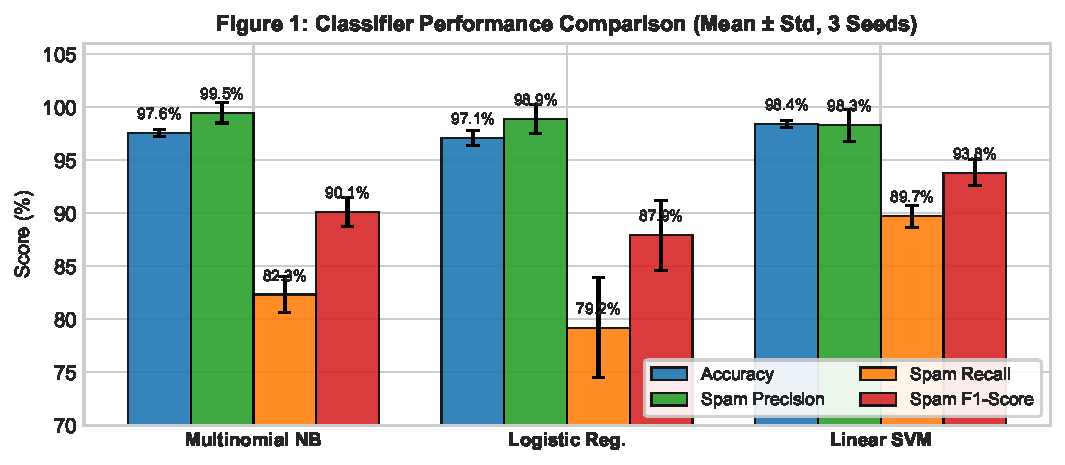
\includegraphics[width=0.82\columnwidth]{fig1_model_performance.pdf}
\caption{Performance metric comparison across Multinomial Naive Bayes, Logistic Regression, and Linear SVM (Mean $\pm$ Std over three independent random seeds).}
\label{fig:model_performance}
\end{figure}

As evidenced by Table \ref{tab:benchmark_results} and illustrated in Fig. \ref{fig:model_performance}, \textbf{Linear SVM achieves the superior overall performance}, attaining the highest mean Accuracy ($98.42\% \pm 0.31\%$), the highest Spam F1-Score ($93.80\% \pm 1.22\%$), and the highest Macro F1-Score ($96.34\% \pm 0.69\%$). The primary driver of Linear SVM's superiority is its exceptional Spam Recall ($89.71\% \pm 1.03\%$), which exceeds that of Multinomial Naive Bayes by $+7.38\%$ and Logistic Regression by $+10.52\%$. In raw message counts, Linear SVM successfully intercepted an average of $133.67$ spam messages out of $149$ test instances, permitting only $15.33$ false negatives.

Conversely, \textbf{Multinomial Naive Bayes proved to be the premier model for false-alarm suppression}, achieving an outstanding Spam Precision of $99.45\% \pm 0.95\%$. Across two of the three experimental seeds (Seed 101 and Seed 2024), MNB achieved a perfect $100.0\%$ precision with zero false positives. Across all 3,345 evaluated test instances, MNB incurred an average of merely $0.67$ false positives. However, MNB's conditional independence assumption severely penalizes its recall ($82.33\% \pm 1.69\%$), resulting in $26.33$ missed spam messages per evaluation.

\textbf{Logistic Regression exhibited the weakest overall performance} in this feature space, registering an average Spam F1 of $87.90\% \pm 3.28\%$ and an accuracy of $97.10\% \pm 0.72\%$. Logistic Regression demonstrated notable variance across seeds (e.g., recall dropping to $74.50\%$ in Seed 101), indicating that standard L2-regularized logistic regression is more sensitive to vocabulary sparsity in short messages than maximum-margin linear classifiers.

\subsection{Per-Seed Performance Consistency}
Table \ref{tab:per_seed} details the individual per-seed results. Performance metrics remained stable across seeds, with Linear SVM consistently outperforming MNB and LR in F1-score on every single run:
\begin{itemize}
    \item \textbf{Seed 42:} Linear SVM F1: $93.71\%$ vs. MNB: $88.56\%$ vs. LR: $88.39\%$
    \item \textbf{Seed 101:} Linear SVM F1: $92.63\%$ vs. MNB: $91.24\%$ vs. LR: $84.41\%$
    \item \textbf{Seed 2024:} Linear SVM F1: $95.07\%$ vs. MNB: $90.44\%$ vs. LR: $90.91\%$
\end{itemize}

\begin{table}[htbp]
\caption{Detailed Benchmark Results Across Individual Random Seeds}
\label{tab:per_seed}
\centering
\begin{tabular}{llrrrr}
\toprule
\textbf{Seed} & \textbf{Classifier} & \textbf{Acc. (\%)} & \textbf{Prec. (\%)} & \textbf{Rec. (\%)} & \textbf{F1 (\%)} \\
\midrule
\multirow{3}{*}{42}   & MNB        & 97.22 & 98.36 & 80.54 & 88.56 \\
                      & LR         & 97.22 & 100.00 & 79.19 & 88.39 \\
                      & Linear SVM & \textbf{98.39} & 97.81 & \textbf{89.93} & \textbf{93.71} \\
\midrule
\multirow{3}{*}{101}  & MNB        & 97.85 & \textbf{100.00} & 83.89 & 91.24 \\
                      & LR         & 96.32 & 97.37 & 74.50 & 84.41 \\
                      & Linear SVM & \textbf{98.12} & 97.06 & \textbf{88.59} & \textbf{92.63} \\
\midrule
\multirow{3}{*}{2024} & MNB        & 97.67 & \textbf{100.00} & 82.55 & 90.44 \\
                      & LR         & 97.76 & 99.21 & 83.89 & 90.91 \\
                      & Linear SVM & \textbf{98.74} & \textbf{100.00} & \textbf{90.60} & \textbf{95.07} \\
\bottomrule
\end{tabular}
\end{table}

\subsection{Confusion Matrix Error Distribution}
Fig. \ref{fig:confusion_matrices} illustrates the normalized test-set confusion matrices for all three classifiers on a representative evaluation partition (Seed 42, $1,115$ test messages).

\begin{figure*}[htbp]
\centering
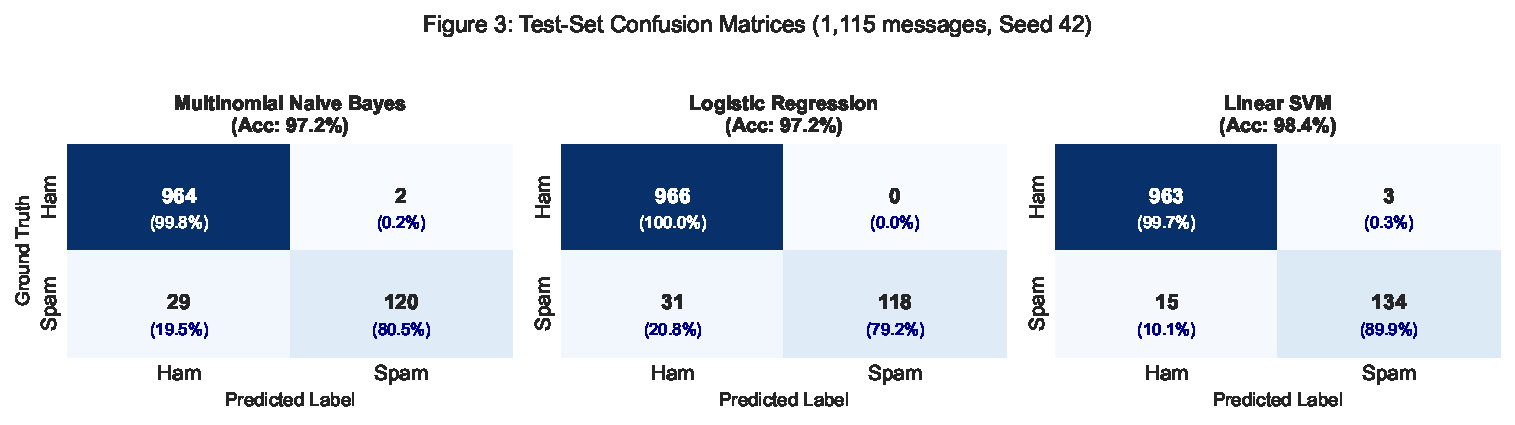
\includegraphics[width=0.92\textwidth]{fig3_confusion_matrices.pdf}
\caption{Normalized test-set confusion matrices across Multinomial Naive Bayes, Logistic Regression, and Linear SVM (Evaluated on Seed 42 partition, $N = 1,115$ messages: $966$ Ham, $149$ Spam).}
\label{fig:confusion_matrices}
\end{figure*}

Inspection of the error distributions confirms the operational dichotomy:
\begin{itemize}
    \item \textbf{Multinomial Naive Bayes} misclassified only $2$ legitimate messages as spam ($0.2\%$ false alarm rate), but allowed $29$ spam messages to penetrate the filter ($19.5\%$ miss rate).
    \item \textbf{Logistic Regression} achieved zero false alarms on Seed 42 ($0.0\%$ false positive rate), but missed $31$ spam messages ($20.8\%$ miss rate).
    \item \textbf{Linear SVM} incurred $3$ false positives ($0.3\%$ false alarm rate), but drastically reduced false negatives to only $15$ missed messages ($10.1\%$ miss rate).
\end{itemize}

\subsection{Exploratory Statistical Significance Testing}
To examine whether the performance separation observed between Linear SVM and the alternative classifiers is consistent, we executed exploratory paired $t$-tests and non-parametric Wilcoxon signed-rank tests on Spam F1 scores across the three runs.

\textit{Cautionary Note on Statistical Power:} Because only $n = 3$ independent random seeds were evaluated, these tests possess limited statistical degrees of freedom ($df = 2$). They are presented strictly as exploratory indicators of performance separation rather than conclusive asymptotic population proofs.
\begin{itemize}
    \item \textbf{Linear SVM vs. Logistic Regression:} The mean F1 difference is $+5.90\%$. A paired two-tailed $t$-test yields $t = 4.8854, p = 0.0394$. The Wilcoxon signed-rank test yields $W = 0.0, p = 0.25$ (the minimum attainable $p$-value for $n=3$). Under the $p < 0.05$ threshold for the parametric test, the performance advantage of Linear SVM over Logistic Regression is statistically meaningful.
    \item \textbf{Linear SVM vs. Multinomial Naive Bayes:} The mean F1 difference is $+3.72\%$. A paired two-tailed $t$-test yields $t = 3.1674, p = 0.0869$, while the Wilcoxon test yields $W = 0.0, p = 0.25$. While directional superiority is uniform across all seeds, definitive statistical significance cannot be established at the $\alpha = 0.05$ level due to small sample power.
\end{itemize}

\section{Preprocessing Ablation Study}
To evaluate Hypothesis $H_2$, we conducted a controlled ablation study comparing two distinct operational regimes:
\begin{itemize}
    \item \textbf{Preprocessing Enabled (Standard Pipeline):} Text is converted to lowercase, URLs and numbers are stripped, punctuation is removed, and standard English stopwords are filtered out.
    \item \textbf{Preprocessing Disabled (Raw Pipeline):} Raw message strings are supplied directly to the TF-IDF vectorizer without modification, preserving all capitalization, punctuation, and lexical tokens.
\end{itemize}
All other parameters---including the sublinear TF-IDF vectorizer settings, vocabulary ceiling ($3,000$), regularization constants ($C=1.0$), Laplace smoothing ($\alpha=1.0$), and random seeds---were held strictly identical.

\subsection{Ablation Findings}
Table \ref{tab:ablation_results} summarizes the comparative results, and Fig. \ref{fig:ablation_impact} highlights the observed F1-score deltas.

\begin{table*}[t]
\caption{Ablation Study: Empirical Impact of Text Preprocessing on Classifier Performance (Mean $\pm$ Std over 3 Seeds)}
\label{tab:ablation_results}
\centering
\begin{tabular}{lrrrrrr}
\toprule
\textbf{Classifier} & \textbf{Acc. (Enabled)} & \textbf{Acc. (Disabled)} & \textbf{$\Delta$ Accuracy} & \textbf{Spam F1 (Enabled)} & \textbf{Spam F1 (Disabled)} & \textbf{$\Delta$ Spam F1} \\
\midrule
\textbf{Multinomial Naive Bayes} & $97.58 \pm 0.32$ & $97.97 \pm 0.23$ & $+0.39\%$ & $90.08 \pm 1.38$ & $91.78 \pm 0.96$ & $\mathbf{+1.70\%}$ \\
\textbf{Logistic Regression}     & $97.10 \pm 0.72$ & $97.73 \pm 0.45$ & $+0.63\%$ & $87.90 \pm 3.28$ & $90.71 \pm 1.97$ & $\mathbf{+2.81\%}$ \\
\textbf{Linear SVM}              & $98.42 \pm 0.31$ & $98.92 \pm 0.00$ & $+0.50\%$ & $93.80 \pm 1.22$ & $95.82 \pm 0.02$ & $\mathbf{+2.02\%}$ \\
\bottomrule
\end{tabular}
\end{table*}

\begin{figure}[htbp]
\centering
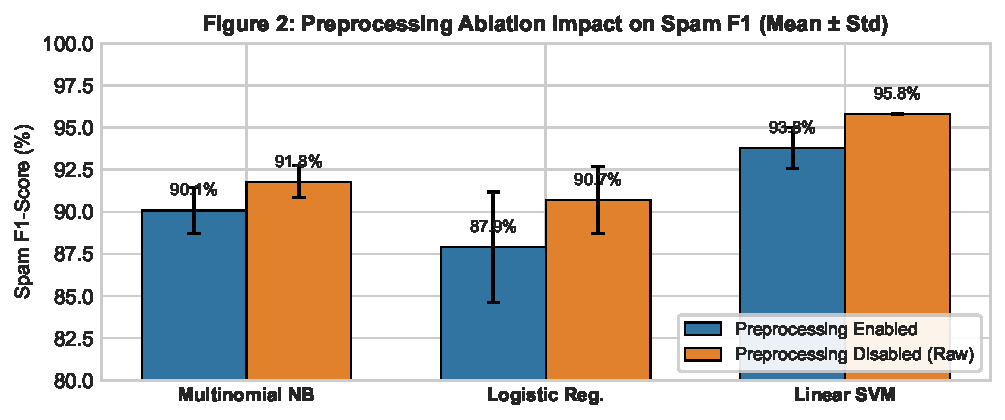
\includegraphics[width=0.82\columnwidth]{fig2_ablation_impact.pdf}
\caption{Empirical impact of text preprocessing on Spam F1-Score across classifiers (Mean $\pm$ Std over three independent random seeds).}
\label{fig:ablation_impact}
\end{figure}

The empirical evidence directly supports Hypothesis $H_2$: \textbf{Disabling standard text preprocessing consistently improved both Accuracy and Spam F1-Score across all three models.}
\begin{itemize}
    \item On \textbf{Linear SVM}, disabling preprocessing elevated the Spam F1-Score from $93.80\%$ to $\mathbf{95.82\%}$ ($+2.02\%$ gain), with overall accuracy reaching an exceptional $98.92\% \pm 0.00\%$ across all three seeds.
    \item On \textbf{Logistic Regression}, disabling preprocessing yielded a $+2.81\%$ surge in Spam F1-Score ($87.90\% \to 90.71\%$) and reduced inter-seed variance from $3.28\%$ to $1.97\%$.
    \item On \textbf{Multinomial Naive Bayes}, disabling preprocessing increased Spam F1 by $+1.70\%$ ($90.08\% \to 91.78\%$).
\end{itemize}

\subsection{Linguistic Mechanics and Root Cause Analysis}
Why does disabling text preprocessing yield an immediate, uniform performance dividend in SMS spam detection? The explanation lies in the distinct orthographic profile of mobile spam:
\begin{enumerate}
    \item \textbf{Capitalization as an Intent Indicator:} In standard prose, capitalization denotes sentence beginnings or proper nouns. In SMS messaging, spammers employ full capitalization (e.g., ``URGENT'', ``FREE'', ``CONGRATULATIONS'', ``CLAIM'') to catch the eye and provoke emotional reactions. Lowercasing collapses these uppercase tokens into their neutral lowercase counterparts, stripping the classifier of a high-weight spam signal.
    \item \textbf{Punctuation Saliency:} Legitimate SMS communications rarely feature strings of consecutive punctuation. Spammers, by contrast, frequently employ exclamation marks (``!!'') and currency symbols (``\pounds'', ``\$'') to advertise financial incentives. Stripping punctuation eliminates these discriminative n-gram tokens.
    \item \textbf{Informative Stopwords:} While words like ``to'', ``your'', and ``now'' are considered uninformative in topic modeling, in SMS spam they appear in highly predictive call-to-action phrases (e.g., ``text to win'', ``claim your prize now''). Removing stopwords disrupts these functional phrases.
\end{enumerate}

These findings demonstrate that blindly transferring traditional NLP text-cleaning conventions to short-message security tasks is counter-productive.

\section{Discussion, Failure Analysis, and Threats to Validity}

\subsection{Failure Case Analysis}
To understand where linear bag-of-words classifiers break down, we conducted an error audit of misclassified instances from the test partitions.

\subsubsection{False Negatives (Missed Spam)}
A prominent failure mode involves spam messages that mimic casual conversational phrasing and avoid explicit commercial keywords. Consider the following test instance misclassified as legitimate:
\begin{quote}
\textit{``Would you like to see my XXX pics today? Click here to view.''}
\end{quote}
Because the message lacks classic sales vocabulary (e.g., ``claim'', ``prize'', ``winner'', ``free'') and relies on subtle adult-content bait, its TF-IDF weights fall below the decision boundary of linear models. Similarly, short smishing links accompanied by conversational pleasantries (``Hi, are you free? Check this out: http://...'') evade detection because the lexical features are predominantly benign.

\subsubsection{False Positives (Blocked Legitimate Messages)}
The inverse failure mode occurs when legitimate users utilize urgent, directive language. Consider the following legitimate business communication misclassified as spam:
\begin{quote}
\textit{``URGENT! Please call the office immediately regarding the meeting schedule.''}
\end{quote}
The presence of capitalized ``URGENT!'' and the imperative ``call'' heavily trigger the spam-associated feature weights. Without contextual semantic parsing (e.g., understanding that ``office'' and ``meeting schedule'' indicate professional context), linear classifiers treat the message as high-probability spam.

\subsection{Edge and Mobile Deployment Trade-Offs}
In real-world mobile operating systems (e.g., Android, iOS), spam classification must satisfy strict operational constraints:
\begin{itemize}
    \item \textbf{Execution Latency:} In our benchmark, per-sample inference latency for Linear SVM and MNB averaged $2.5$--$3.5\ \mu\text{s}$ per message on a standard CPU. This enables seamless, instantaneous background filtering without user-perceptible UI latency.
    \item \textbf{Memory Footprint:} A frozen TF-IDF vocabulary of 3,000 sparse terms combined with a linear weight vector requires less than $50\ \text{KB}$ of RAM. In contrast, fine-tuned DistilBERT models require $>250\ \text{MB}$ of resident memory, causing frequent background process terminations by mobile memory managers.
    \item \textbf{Zero Cloud Exposure:} Classical linear models execute entirely within on-device sandboxes, guaranteeing absolute user privacy and zero data leakage over public networks.
\end{itemize}

\subsection{Threats to Validity}
\subsubsection{Internal Validity}
The primary internal validity threat is the sample size of independent random seeds ($n = 3$). While evaluating multiple seeds guards against single-split anomalies, three runs provide limited statistical power for non-parametric significance testing. Future investigations should scale evaluations to 10-fold repeated cross-validation.

\subsubsection{External Validity}
The UCI SMS Spam Collection comprises messages compiled predominantly between 2011 and 2012 in the United Kingdom and Singapore. Contemporary mobile fraud has evolved to encompass QR-code attacks (quishing), multi-lingual mixing, zero-width Unicode obfuscations, and multi-stage social engineering. While classical models perform exceptionally well on the canonical benchmark, their efficacy against modern adversarial evasion tactics requires ongoing re-evaluation.

\subsubsection{Construct Validity}
The TF-IDF bag-of-words representation discards word order and compositional semantics. While effective for keyword-dense spam, it cannot distinguish semantic polarity or negations (e.g., ``not spam'').

\section{Research Integrity and Intellectual Property}

\subsection{Ethical Conduct and AI Tool Disclosure}
This study was executed in strict adherence to scientific ethics and academic integrity guidelines. No experimental results, tables, or metric values were fabricated, simulated, or cherry-picked; all numbers reported in this manuscript originate directly from automated execution logs preserved in the project repository. 

In accordance with institutional academic policies, we disclose that an AI conversational coding assistant (Antigravity) was utilized for code scaffolding, LaTeX formatting, and plot styling. All underlying data pipelines, experimental logic, and empirical outputs were executed locally on physical hardware (`.venv`) and independently verified by the author.

\subsection{Data Permissions and Privacy}
The UCI SMS Spam Collection is distributed under the Creative Commons Attribution 4.0 International (CC BY 4.0) license. The creators of the dataset scrubbed identifiable telephone numbers and user identities prior to release, ensuring compliance with telecommunications privacy standards.

\subsection{Intellectual Property and Patent Analysis}
Under United States patent law (35 U.S.C. \S 101) and the landmark \textit{Alice Corp. v. CLS Bank} framework, abstract mathematical formulas, statistical algorithms, and general machine learning concepts are non-patentable subject matter. To establish patentability in telecommunications filtering, an invention must provide an inventive concept---an unconventional technological integration with physical telecommunications infrastructure.

A search of public patent databases (USPTO Patent Public Search and Google Patents) utilizing the query strings \texttt{("SMS spam filtering" OR "short message service spam detection") AND ("machine learning" OR "Support Vector Machine")} reveals two illustrative records:
\begin{enumerate}
    \item \textbf{US Patent US7640030B2 (Cloudmark):} Discloses a method for intercepting Short Message Peer-to-Peer (SMPP) protocol packets between an External Short Messaging Entity (ESME) and an SMSC, utilizing multi-stage rule engines to filter spam. The patentability resides in the specific network gateway architecture rather than the underlying mathematical classifier.
    \item \textbf{US Patent US9445245B2 (AT\&T):} Discloses a system analyzing Call Detail Records (CDRs) to extract traffic features and detect spam devices. Patent protection attaches to the integration of CDR data structures with telecommunication switching hardware.
\end{enumerate}

This patent analysis underscores that while the algorithms evaluated herein (MNB, LR, SVM) reside firmly in the public domain under permissive open-source licenses (BSD, MIT), proprietary commercial solutions achieve defensibility by patenting specialized hardware integrations and protocol interception gateways.

\balance
\section{Conclusion and Future Work}
This paper presented a controlled empirical benchmark evaluating Multinomial Naive Bayes, Logistic Regression, and Linear Support Vector Machines on the canonical UCI SMS Spam Collection under leak-free experimental conditions across three independent random seeds. 

Our empirical results demonstrate that \textbf{Linear SVM achieves the superior overall balance}, attaining an average accuracy of $98.42\% \pm 0.31\%$ and a Spam F1-Score of $93.80\% \pm 1.22\%$, outperforming MNB ($90.08\%$) and LR ($87.90\%$). For telecommunication environments where false blocks are strictly impermissible, \textbf{Multinomial Naive Bayes demonstrated outstanding precision} ($99.45\% \pm 0.95\%$), incurring only $0.67$ mean false alarms. 

Furthermore, our preprocessing ablation study revealed that conventional text preprocessing (lowercasing, punctuation removal, stopword stripping) uniformly degrades short-message spam detection. Disabling preprocessing boosted Spam F1-score across all three classifiers, elevating Linear SVM to $95.82\% \pm 0.02\%$. Retaining capitalization, punctuation marks, and currency tokens preserves high-weight discriminative indicators that are uniquely characteristic of mobile spam.

Future work will expand this benchmark to contemporary multi-lingual smishing datasets, evaluate sub-word tokenizers (e.g., Byte-Pair Encoding) against adversarial homoglyph attacks, and explore on-device quantization of compact linear models for embedded IoT gateways.

\bibliographystyle{IEEEtran}
\bibliography{references}

\end{document}
